% USE PDFLatex!
% to correctly render Swedish characters

\documentclass{popsci}

\usepackage[utf8]{inputenc}
\usepackage[swedish, english]{babel}

\usepackage{fancyhdr}
\usepackage{titling}
\usepackage{color}
\usepackage{colortbl}
\usepackage{graphicx}
\usepackage{flushend}
\usepackage{lmodern}


% Please specify the presentation date
\presentationsdag{2022-06-07}

% use either of these commands to specify the title of your thesis
\examensarbete{Drones for Sea Rescue: Lab and Field Experiments on Camera Gimbal Control}
% To create a title in two rows, leave examensarbete blank and fill in examensarbeteTwoRows.
%\examensarbeteTwoRows{}{}
\student{Alexander Sandström}
%\students{Magnus Hultin}{Mr X}
\supervisor{William Tärneberg (LTH), Fredrik Falkman (Sjöräddningssällskapet)}
\examiner{Maria Kihl(LTH)}

% Your pop-sci title should be different (more catchy) than your thesis title
\title{Drönare som understöd vid sjöräddning}


\begin{document}

% not more than 4 rows!
%\theabstract{Applikations-specifika processorer är allt mer vanligt för få ut rätt prestanda med så lite resurser som möjligt. Detta arbete har en parametrisk modell för att kunna testa hur mycket resurser som behövs för en specifik applikation.}
\theabstract{Sjöräddningssällskapet (SSRS) driver idag ett projekt där man utforskar möjligheten att använda drönare för att understödja räddningspersonal vid uttryckning till havs. I detta examensarbete har en mjukvara för att styra en drönarkamera implementerats. Den har sedan utvärderats i labb och under riktig flygning.}

{\noindent Vid en uttryckning till havs kan små skillnader i tid vara avgörande för om en utryckning resulterar i en lyckad räddning eller en katastrof. För att kunna ge räddningspersonalen bättre beslutsunderlag i ett så tidigt skede som möjligt driver SSRS ett innovationsprojekt kallat Eyes-On-Scene (EOS), där man undersöker användningen av drönare inom sjöräddning. Drönarna ska vara stationerade längs kusten och kunna skickas ut direkt vid ett larm för att sedan skicka bilder till sjöräddarna på väg till olyckan.

\begin{figure}[!bth] % Use pictures in your pop-vet!
    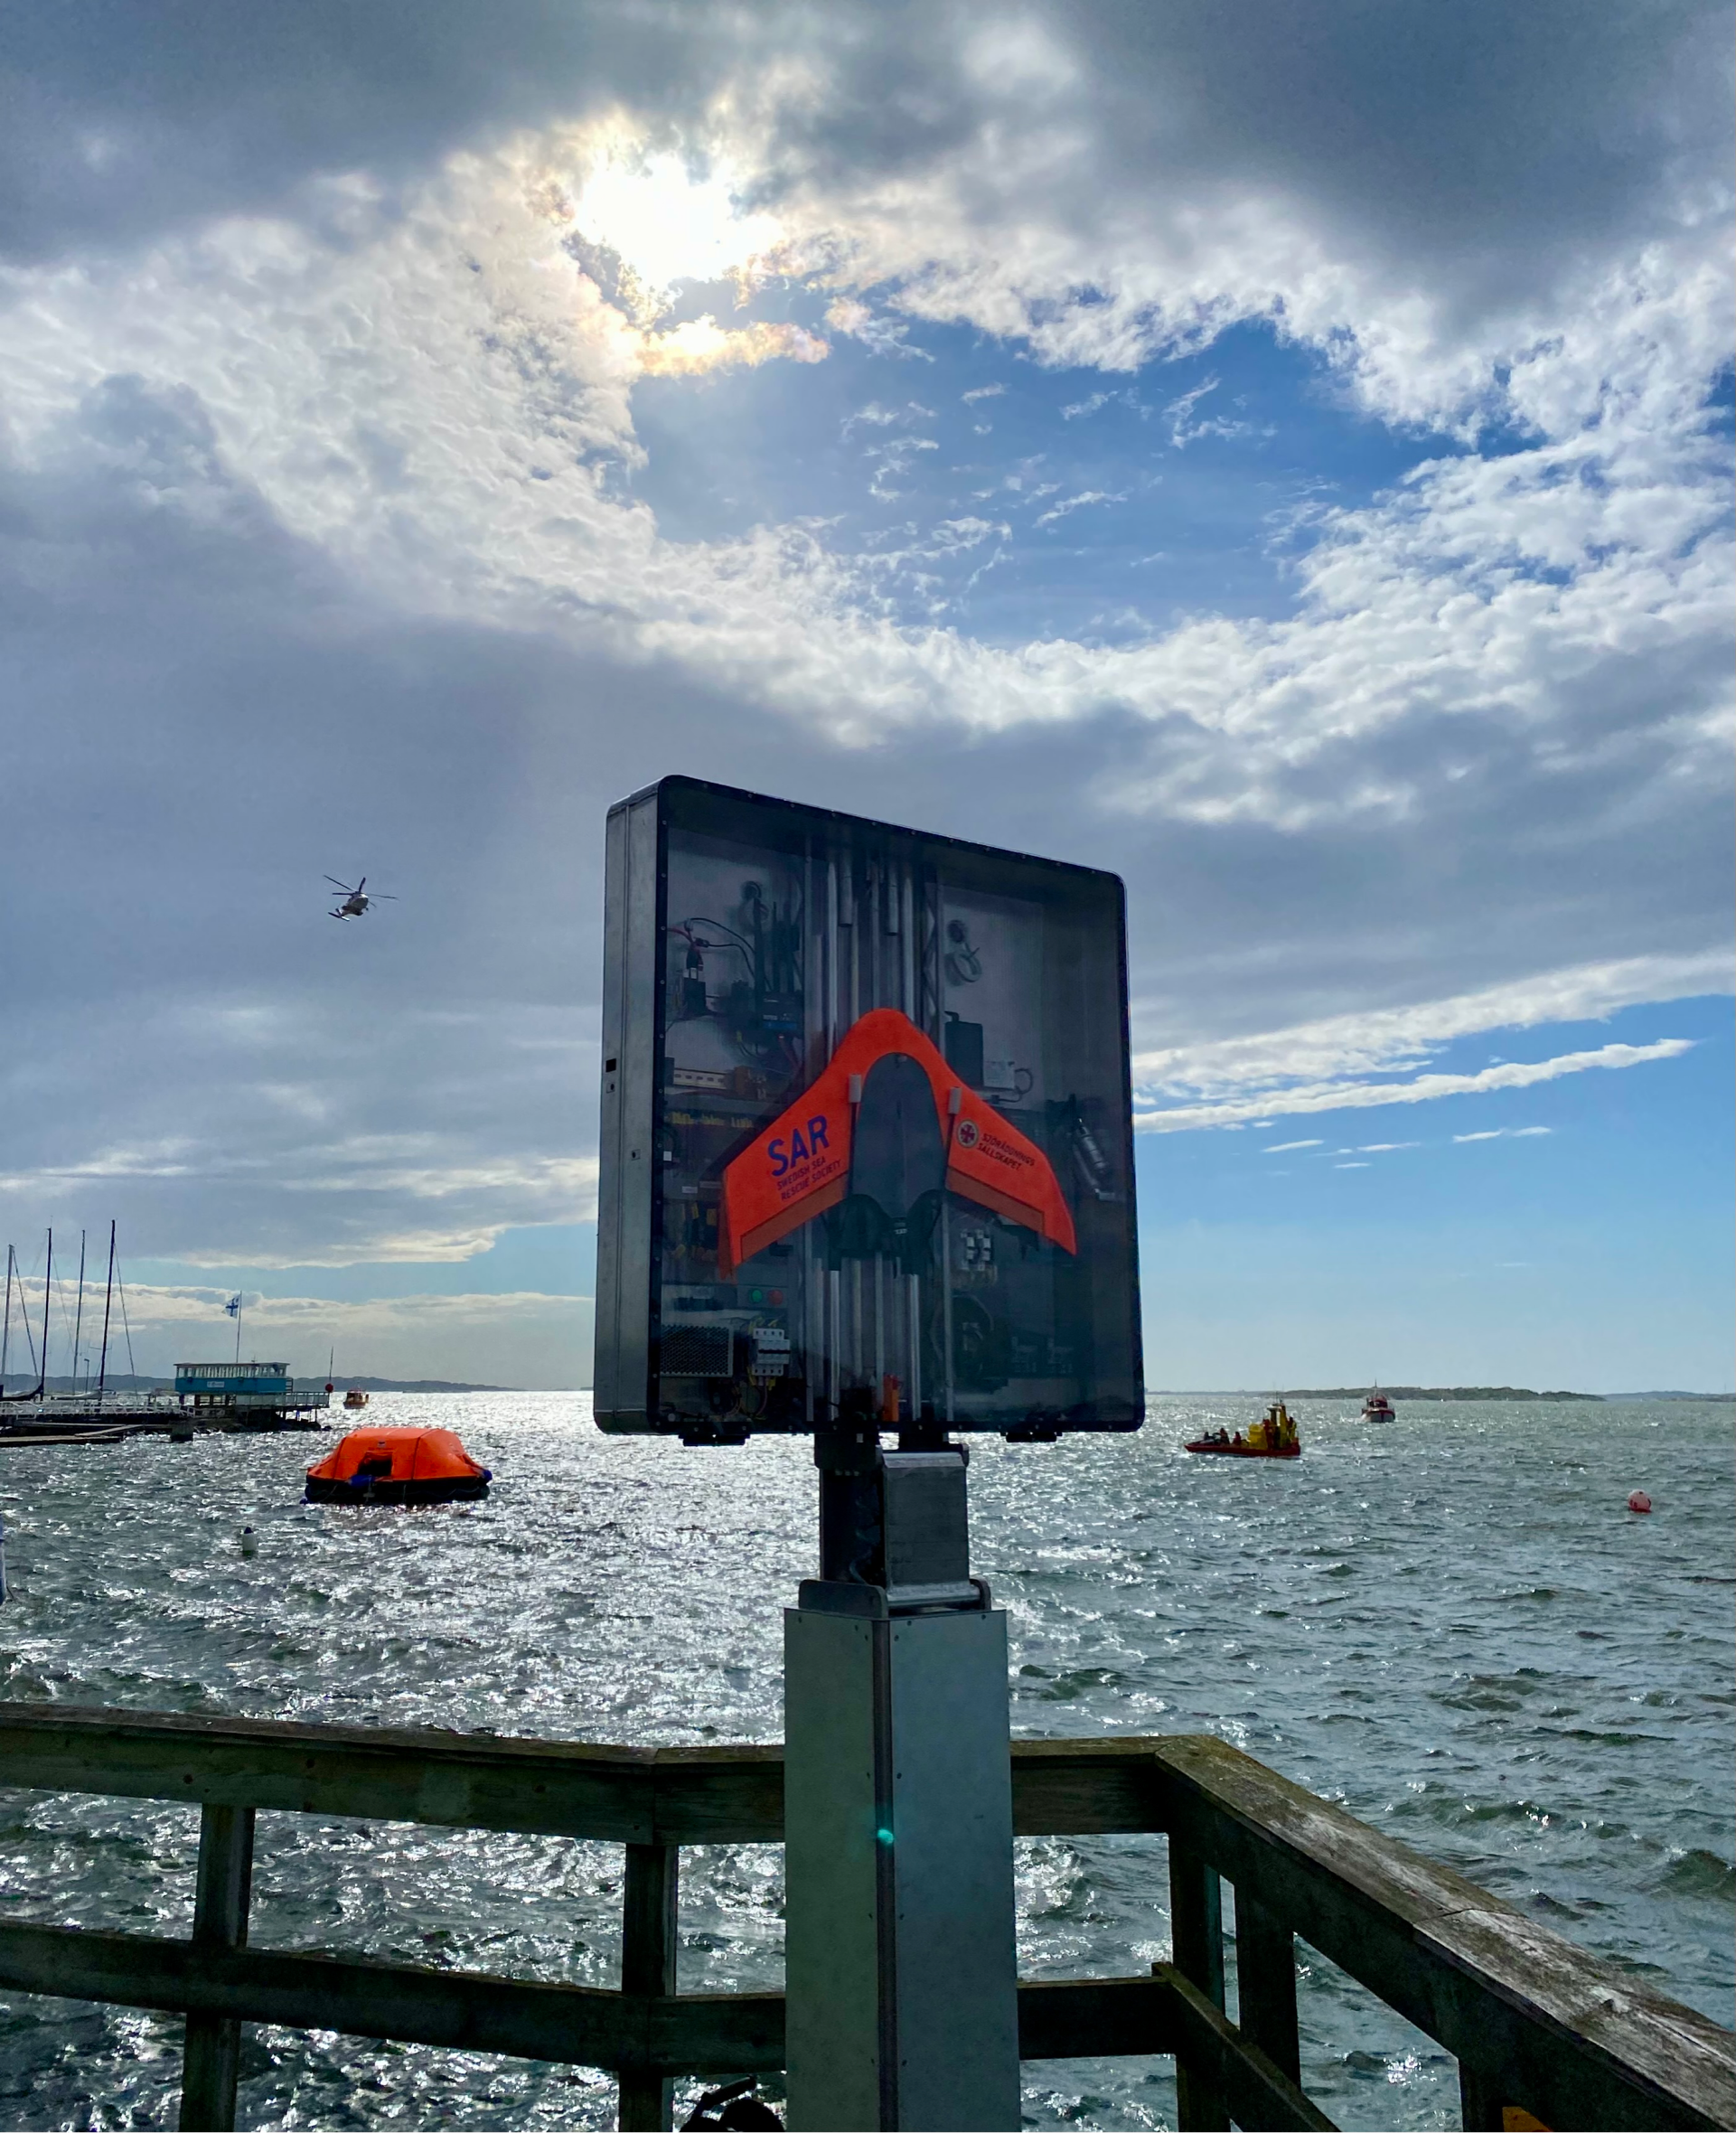
\includegraphics[trim={0 20cm 0 30cm},width=\columnwidth, clip]{../images/dronepic.png} 
    %\caption{En fin bild}
\end{figure}

Den drönare som tagits fram i projektet är en så kallad fastvinge, som är en snabbare och mer energieffektiv konstruktion än den mer vanliga rotordrönaren. Den har även ett 4G-modem, vilket gör att den kan styras över Internet, varifrån som helst på jorden. 

Drönarens enda verktyg är en gimbalmonterad kamera, som under flygning styrs genom att sätta ut GPS-punkter som drönaren då automatiskt riktar kameran mot. Då det inte alltid är lätt att trycka rätt på en karta har det varit svårt att få kameran att kolla på det man vill kolla på, och SSRS har därför varit ute efter ett snabbare sätt att justera kameravyn.

I mitt examensarbete har jag utvecklat ett gränsnitt för att styra drönarkameran med en joystick. Jag har sedan i en labbmiljö undersökt hur olika fördröjningar påverkar en kameraoperatör som använder gränsittet. Mjukvaran har sedan integrerats med EOS-drönarens system för att kunna styra kameran under en riktig flygning, och flera lyckade testflygningar genomfördes. 

Resultaten visar att fördröjning försämrar både operatörens prestation och upplevelse, men att sambanden är olika. Exempelvis tyder resultaten på att vissa nivåer av fördröjningar kan försämra operatörens prestation mer än upplevelsen, och att det omvända verkar gälla för andra nivåer av fördröjningar.

Testbädden visar potential i vidare studier i operatörsupplevelse, som blir ett allt mer relevant område då fler områden tillämpar fjärrstyrning. Mjukvaran kommer även användas av SSRS i framtida flygningar, där man i år förbereder för skarp utryckning för första gången i projektet.
}
\end{document}
